\chapter{Aplikacja - symulator}
\label{ch:dodatekA-aplikacja}
\section{Założenia projektowe aplikacji}
\section{Instrukcja instalacyjna}
\section{Opis interfejsu graficznego}

\par
Wygląd aplikacji przedstawiono na rysunku \ref{fig:app01-fullScreen}. Interfejs można podzielić funkcjonalnie na 5 części oznaczonych \emph{A}, \emph{B}, \emph{C} i \emph{D} oraz osobno przedstawionej na rysunku \ref{fig:app01-plotTab}. 

\par
Sekcja \emph{A} pozwala na zdefiniowanie i wywołanie operacji. Możliwe jest uruchomienie zarówno procesu selekcji parametrów algorytmów jak i badań pod kątem jednego z kryteriów porównawczych użytych w pracy. Możliwy jest wybór spośród trzech funkcji testowych lub zdefiniowanej przez użytkownika - opcja \emph{(code)}. Lista z prawe strony panelu umożliwia na określenie, które z scenariuszy doboru parametrów powinny zostać użyte do selekcji. Możliwością dostępną jedynie w przypadku wykorzystania funkcji \emph{Schaffer nr 2} lub własnej funkcji z dwoma parametrami jest wygenerowanie jej wykresu w dziedzinie równej zakresowi poszczególnych atrybutów. 

\par
Panel oznaczony jako \emph{B} przedstawia bieżące konfiguracje algorytmów, które zostaną wykorzystane w przypadku uruchomienia badań porównawczych. Przy starcie aplikacji parametry wszystkich mechanizmów ustawiane są na te uzyskane w trakcie badań dla funkcji \emph{Schaffer nr 2}.

\par
Przedstawiona na rysunku \ref{fig:app01-fullScreen} sekcja \emph{C} przedstawia panel umożliwiający definiowanie własnych funkcji testowych. Górna część pozwala na określenie liczby, nazwy i zakresu parametrów. Przycisk \emph{Generate} tworzy pusty szablon w oparciu o określone parametry. Kod źródłowy opisujący nową funkcję należy zapisać w języku \emph{R}. W wskazanym polu edycji możliwe jest definiowanie dodatkowych pomocniczych funkcji jak również i dołączanie konkretnych pakietów. Nie można jednak modyfikować nazwy funkcji, ponieważ będzie to skutkowało niepoprawnym działaniem aplikacji. Zakładka \emph{code} aktywna jest jedynie wtedy, gdy w panelu \emph{A} wybrano opcję \emph{(code)}.

\par
Dolna część \emph{D} aplikacji stanowi narzędzie pomocnicze dla użytkownika. Zamieszczane są tam logi aplikacji umożliwiające rozwiązywanie problemów z poprawnością zdefiniowanej funkcji. Dodatkowo można znaleźć tam informacje dotyczące lokalizacji w systemie plików wykresów powstałych w skutek operacji z panelu \emph{A}. 


\begin{figure}[hbt]
\centering
  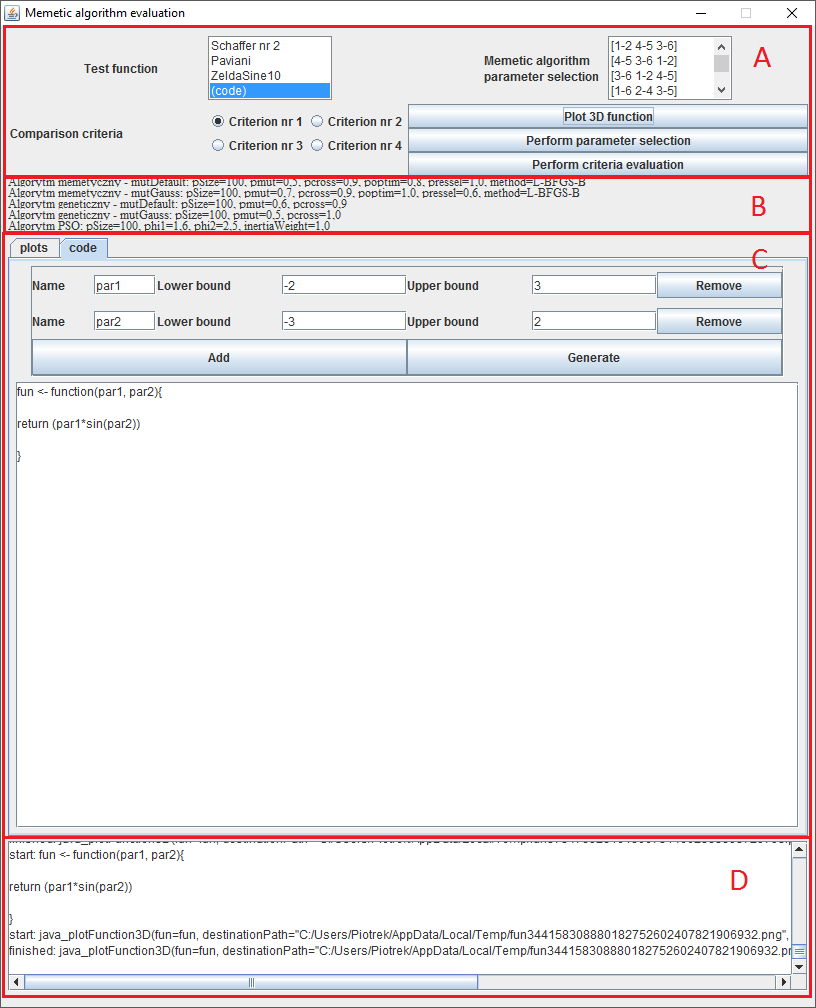
\includegraphics[width=\linewidth]{{img//app01//mockup-with-parts.png}}
\caption{Pełny widok aplikacji}	
\label{fig:app01-fullScreen}
\end{figure}

\par
Na rysunku \ref{fig:app01-plotTab} przedstawiono panel prezentujący wykresy generowane przez aplikację. Przyciskami \emph{Previous} i \emph{Next} możliwe jest przeglądanie pełnej historii wykresów od uruchomienia aplikacji. Jest to ważne z uwagi na fakt, że w wynikiem części operacji może być więcej niż jeden wykres jednocześnie. 

\begin{figure}[hbt]
\centering
  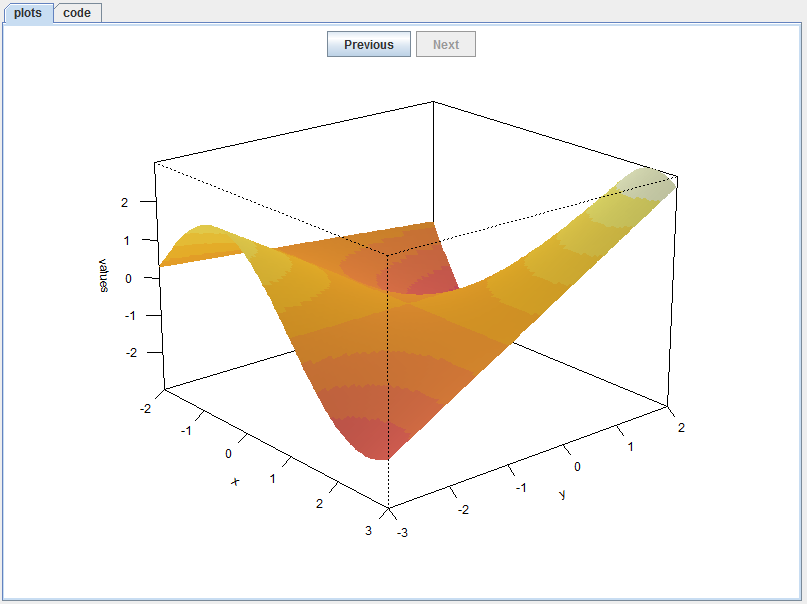
\includegraphics[width=\linewidth]{{img//app01//mockup-plot-tab.png}}
\caption{Zakładka wykresów}	
\label{fig:app01-plotTab}
\end{figure}


